% slides-exemplo-beamer
%
% Sáb Out  1 19:47:43 BRT 2011

\documentclass[table, usenames, svgnames, dvipsnames]{beamer}
\usepackage{beamerthemeshadow}
\usepackage[portuguese]{babel}
\usepackage[latin1]{inputenc}
\usepackage[absolute,overlay]{textpos}
\usepackage{array}

%\usepackage{subfigure}
%\usepackage{multicol}
%\usepackage{colortbl}

% ---------------------------------------------------------------------------- %
% Definições beamer
% ---------------------------------------------------------------------------- %
\usetheme{Rochester}
%\usetheme{Luebeck}
\usecolortheme{rose}

% Algumas definições para o layout
\setbeamerfont{frametitle}{size=\normalsize}
\setbeamerfont{title}{size=\normalsize}
\beamertemplatenavigationsymbolsempty

% Podem ser utilizadas imagens no background
%\setbeamercolor{frametitle}{bg=black}
%\usebackgroundtemplate{\includegraphics[height=\paperheight]{figuras/back.jpg}}

% Os simbolos de navegacao nao sao necessarios
\setbeamertemplate{navigation symbols}{}
\setbeamertemplate{footline}{}

%\setbeamertemplate{footline}[page number]{}
%\setbeamertemplate{footline}[text line]{ \hfill {\insertframenumber}}

% Indice para cada seção (aparece antes de cada section)
\AtBeginSection[] 
{
	\begin{frame}<handout:0>
		\frametitle{\textbf{Agenda}}
		\footnotesize{ \tableofcontents[currentsection,hideothersubsections] }
	\end{frame}
}

% ---------------------------------------------------------------------------- %
% Declarações
% ---------------------------------------------------------------------------- %
\DeclareGraphicsExtensions{.pdf,.jpg,.png} % compilamos apenas com pdflatex
\graphicspath{{./figuras/}} % caminho onde as figuras estarao disponiveis

% Logotipo no canto superior direito
\setlength{\TPHorizModule}{1mm}
\setlength{\TPVertModule}{1mm}
\newcommand{\MyLogo}{%
\begin{textblock}{}(118.5, 2.5)
	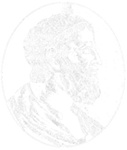
\includegraphics[width=0.7cm]{ime-mod2.png}
\end{textblock}
}

% semitransparente
\newcommand{\semitransp}[2][35]{\color{fg!#1}#2}

% \definecolor{myred}{rgb}{0.8, 0.3, 0.3}
\definecolor{myblue}{rgb}{0.2, 0.2, 0.70196}

\usepackage{framed} % utilizado para codigo fonte
\definecolor{shadecolor}{named}{LightGray} 

% ---------------------------------------------------------------------------- %
% Título
% ---------------------------------------------------------------------------- %
\title{\textbf{Aplicações práticas em técnicas de reconstrução 3D utilizando fotogrametria}}

\author[Pedro Felipe Pena Barata]{\scriptsize
    Pedro Felipe Pena Barata
}

\subtitle{}

\institute{\\[1.0mm] 
Instituto Politécnico do Rio De Janeiro (IPRJ)\\
Universidade do Estado do Rio de Janeiro}

\date{{\tiny 27 de Novembro de 2017}}


% ---------------------------------------------------------------------------- %
\begin{document}
% ---------------------------------------------------------------------------- %

% ---------------------------------------------------------------------------- %
% Primeira página: slide 0
% ---------------------------------------------------------------------------- %

{%\usebackgroundtemplate{}} 
\begin{frame}[plain]

	\begin{columns}[c]
		\column{0.2\textwidth}
			\hspace*{+0.5em}
			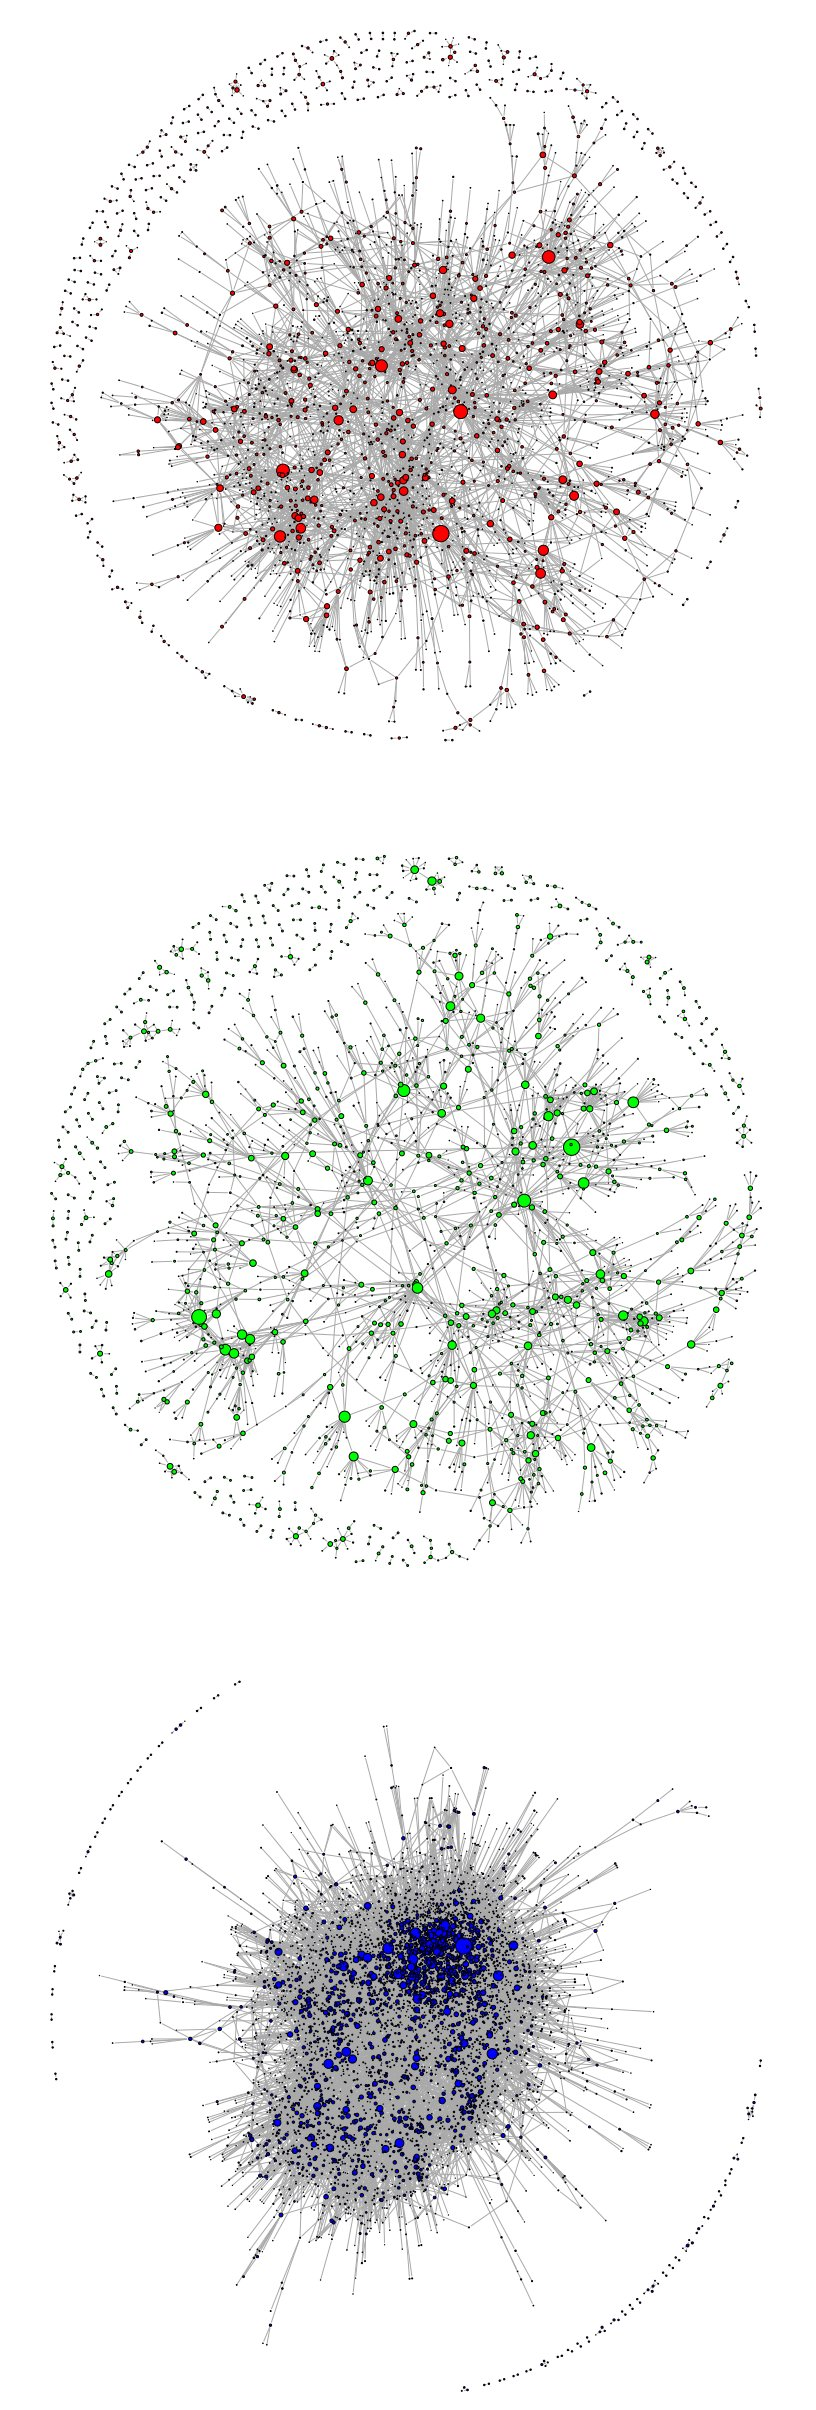
\includegraphics[height=7.90cm]{rede.jpg}
		\column{0.01\textwidth}
		\column{0.70\textwidth}
			\titlepage
	\end{columns}
	\addtocounter{framenumber}{-1}
\end{frame}
}


% ---------------------------------------------------------------------------- %
% slide 1 >
% ---------------------------------------------------------------------------- %
\setbeamertemplate{footline}{\hrule \MyLogo } %\hfill\includegraphics[height=1.2cm]{figuras/olho1.png}}
%\setbeamertemplate{footline}{\hfill\includegraphics[height=1.2cm]{figuras/olho1.png}}
\setbeamertemplate{navigation symbols}{\large {\insertframenumber}}

% ---------------------------------------------------------------------------- %
\begin{frame}[plain]
\frametitle{}
	\hspace*{-0.6cm}
	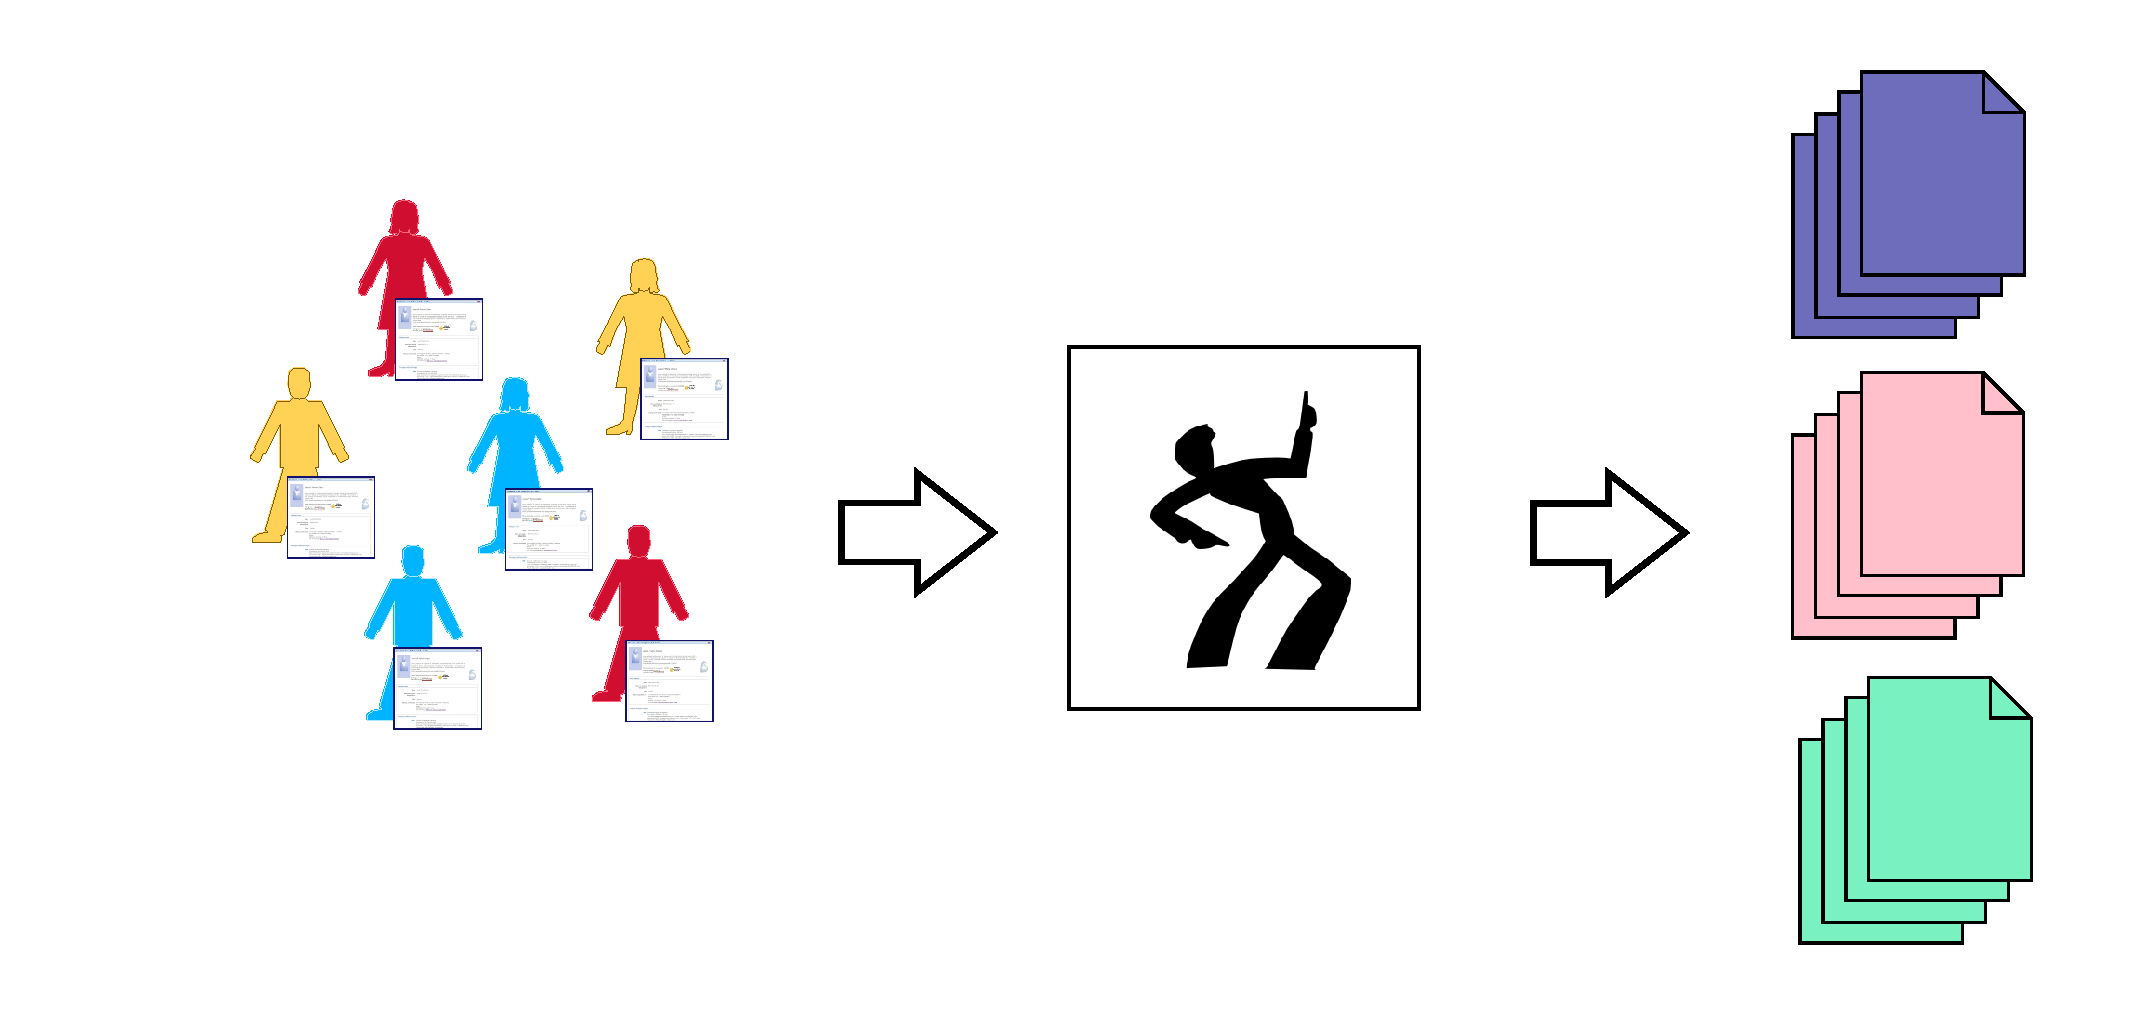
\includegraphics[width=1.1\textwidth]{sota.pdf}
\end{frame}

% \begin{frame}[plain]
% \frametitle{}
% 	\begin{block}{Algumas perguntas interessantes ...}
% 		\begin{enumerate}
% 			\item Questão 1 ...
% 			\item Questão 2 ...
% 			\item Questão 3 ...
% 			\item Questão 4 ...
% 			\item Questão 5 ...
% 			\item Questão 6 ...
% 			\item Questão 7 ...
% 	\end{enumerate}
% 	\end{block}
% \end{frame}

% ---------------------------------------------------------------------------- %
\begin{frame}
\frametitle{\textbf{Agenda}}

	\hspace*{+4.0em}
	\footnotesize{ \tableofcontents }
\end{frame}


% ---------------------------------------------------------------------------- %
\section{Introdução}
% ---------------------------------------------------------------------------- %

\begin{frame} 
\frametitle{\textbf{Cabeçalho...}}
A reconstrucão 3D de cenas gerais a partir de múltiplos pontos de vista usando-se
câmeras convencionais, sem aquisição controlada, é um dos grandes objetivos de pesquisa
em visão computacional, ambicioso até mesmo para os dias de hoje. 
%Os desafios estão ligados às escolhas de grande escala de representações adequadas
% e de técnicas que possam modelar simultaneamente com materiais drasticamente dife-
% rentes (e.g., não-Lambertianos), modelos geométricos (e.g., variedades curvilı́neas gerais,
% descontinuidades, texturas, deformações, em escalas diferentes), tipos de regiões (com ou
% sem textura), condições de iluminação variadas, sombras, fortes diferenças de perspecti-
% vas, desbalanceamento devido a excesso de detalhes em partes menos importantes, número
% arbitrário de objetos e câmeras não-calibradas.

%COLOCAR IMAGEM IMPRESSORA 3D%

\end{frame}

% ---------------------------------------------------------------------------- %
\subsection{Objetivos}
% ---------------------------------------------------------------------------- %

\begin{frame} 
\frametitle{\textbf{Cabeçalho...}}
	\begin{center}
		O objetivo deste trabalho é, por meio de técnicas fotogramétricas, preservar o patrimônio cultural 
		do Jardim do Nêgo, localizado na estrada Teresópolis-Friburgo, Rio de Janeiro. Na qual algumas esculturas 
		foram 
	\end{center}
\end{frame}

% ---------------------------------------------------------------------------- %
\section{Reconstrução à laser}
% ---------------------------------------------------------------------------- %

% ---------------------------------------------------------------------------- %
\subsection{Introdução}
% ---------------------------------------------------------------------------- %

\begin{frame} 
\frametitle{\textbf{Cabeçalho...}}
	\begin{center}
		Texto texto texto texto texto texto texto texto texto texto texto texto texto
		texto texto texto.
	\end{center}
\end{frame}

% ---------------------------------------------------------------------------- %
\subsection{Esculturas de Michelangelo}
% ---------------------------------------------------------------------------- %

\begin{frame} 
\frametitle{\textbf{Cabeçalho...}}
	\begin{center}
		Texto texto texto texto texto texto texto texto texto texto texto texto texto
		texto texto texto.
	\end{center}
\end{frame}

% ---------------------------------------------------------------------------- %
\section{Kinect}
% ---------------------------------------------------------------------------- %

\begin{frame}
\frametitle{Cabeçalho...}
	\begin{enumerate}
    	\item Texto texto texto texto texto texto texto texto...
		\\[0.5em]

    	\item Texto texto texto texto texto texto texto texto...
		\\[0.5em]
    	
		\item Texto texto texto texto texto texto texto texto...
		\\[0.5em]
	\end{enumerate}
\end{frame}

% ---------------------------------------------------------------------------- %
\subsection{Introdução}
% ---------------------------------------------------------------------------- %

\begin{frame} 
\frametitle{\textbf{Cabeçalho...}}
	\begin{center}
		Texto texto texto texto texto texto texto texto texto texto texto texto texto
		texto texto texto.
	\end{center}
\end{frame}

% ---------------------------------------------------------------------------- %
\subsection{Kinect com \emph{Structure from Motion}}
% ---------------------------------------------------------------------------- %

\begin{frame} 
\frametitle{\textbf{Cabeçalho...}}
	\begin{center}
		Texto texto texto texto texto texto texto texto texto texto texto texto texto
		texto texto texto.
	\end{center}
\end{frame}

% ---------------------------------------------------------------------------- %
\section{\emph{Structure from Motion}}
% ---------------------------------------------------------------------------- %

\begin{frame}
\frametitle{Cabeçalho...}
	\begin{enumerate}
    	\item Texto texto texto texto texto texto texto texto...
		\\[0.5em]

    	\item Texto texto texto texto texto texto texto texto...
		\\[0.5em]
    	
		\item Texto texto texto texto texto texto texto texto...
		\\[0.5em]
	\end{enumerate}
\end{frame}

% ---------------------------------------------------------------------------- %
\subsection{Introdução}
% ---------------------------------------------------------------------------- %

\begin{frame} 
\frametitle{\textbf{Cabeçalho...}}
	\begin{center}
		Texto texto texto texto texto texto texto texto texto texto texto texto texto
		texto texto texto.
	\end{center}
\end{frame}

% ---------------------------------------------------------------------------- %
\subsection{MVE -- \emph{Multi-View Stereo Environment}}
% ---------------------------------------------------------------------------- %

\begin{frame} 
\frametitle{\textbf{Cabeçalho...}}
	\begin{center}
		Texto texto texto texto texto texto texto texto texto texto texto texto texto
		texto texto texto.
	\end{center}
\end{frame}

% ---------------------------------------------------------------------------- %
\subsubsection{\emph{dmrecon}}
% ---------------------------------------------------------------------------- %

\begin{frame} 
\frametitle{\textbf{Cabeçalho...}}
	\begin{center}
		Texto texto texto texto texto texto texto texto texto texto texto texto texto
		texto texto texto.
	\end{center}
\end{frame}

% ---------------------------------------------------------------------------- %
\subsubsection{\emph{FSSRecon}}
% ---------------------------------------------------------------------------- %

\begin{frame} 
\frametitle{\textbf{Cabeçalho...}}
	\begin{center}
		Texto texto texto texto texto texto texto texto texto texto texto texto texto
		texto texto texto.
	\end{center}
\end{frame}


% ---------------------------------------------------------------------------- %
\subsection{VisualSfM}
% ---------------------------------------------------------------------------- %

\begin{frame} 
\frametitle{\textbf{Cabeçalho...}}
	\begin{center}
		Texto texto texto texto texto texto texto texto texto texto texto texto texto
		texto texto texto.
	\end{center}
\end{frame}

% ---------------------------------------------------------------------------- %
\subsubsection{PBA/MCBA -- \emph{Parallel Bundle Adjustment/Multi-core Bundle Adjustment}}
% ---------------------------------------------------------------------------- %

\begin{frame} 
\frametitle{\textbf{Cabeçalho...}}
	\begin{center}
		Texto texto texto texto texto texto texto texto texto texto texto texto texto
		texto texto texto.
	\end{center}
\end{frame}

% ---------------------------------------------------------------------------- %
\subsubsection{CMVS/PMVS-2 -- \emph{Clustering Views for Multi-view Stereo / Patch-based for Multi-view Stereo version 2}}
% ---------------------------------------------------------------------------- %

\begin{frame} 
\frametitle{\textbf{Cabeçalho...}}
	\begin{center}
		Texto texto texto texto texto texto texto texto texto texto texto texto texto
		texto texto texto.
	\end{center}
\end{frame}

% ---------------------------------------------------------------------------- %
\section{Experimentos}
% ---------------------------------------------------------------------------- %

\begin{frame}
\frametitle{Cabeçalho...}
	\begin{enumerate}
    	\item Texto texto texto texto texto texto texto texto...
		\\[0.5em]

    	\item Texto texto texto texto texto texto texto texto...
		\\[0.5em]
    	
		\item Texto texto texto texto texto texto texto texto...
		\\[0.5em]
	\end{enumerate}
\end{frame}

% ---------------------------------------------------------------------------- %
\subsection{VisualSfM}
% ---------------------------------------------------------------------------- %

\begin{frame}
\frametitle{Cabeçalho...}
	\begin{enumerate}
    	\item Texto texto texto texto texto texto texto texto...
		\\[0.5em]

    	\item Texto texto texto texto texto texto texto texto...
		\\[0.5em]
    	
		\item Texto texto texto texto texto texto texto texto...
		\\[0.5em]
	\end{enumerate}
\end{frame}

% ---------------------------------------------------------------------------- %
\subsubsection{Escultura do Jardim do Nêgo}
% ---------------------------------------------------------------------------- %

\begin{frame}
\frametitle{Cabeçalho...}
	\begin{enumerate}
    	\item Texto texto texto texto texto texto texto texto...
		\\[0.5em]

    	\item Texto texto texto texto texto texto texto texto...
		\\[0.5em]
    	
		\item Texto texto texto texto texto texto texto texto...
		\\[0.5em]
	\end{enumerate}
\end{frame}

% ---------------------------------------------------------------------------- %
\subsubsection{Objeto em ambiente fechado}
% ---------------------------------------------------------------------------- %

\begin{frame}
\frametitle{Cabeçalho...}
	\begin{enumerate}
    	\item Texto texto texto texto texto texto texto texto...
		\\[0.5em]

    	\item Texto texto texto texto texto texto texto texto...
		\\[0.5em]
    	
		\item Texto texto texto texto texto texto texto texto...
		\\[0.5em]
	\end{enumerate}
\end{frame}


% ---------------------------------------------------------------------------- %
\subsection{MVE}
% ---------------------------------------------------------------------------- %

\begin{frame}
\frametitle{Cabeçalho...}
	\begin{enumerate}
    	\item Texto texto texto texto texto texto texto texto...
		\\[0.5em]

    	\item Texto texto texto texto texto texto texto texto...
		\\[0.5em]
    	
		\item Texto texto texto texto texto texto texto texto...
		\\[0.5em]
	\end{enumerate}
\end{frame}

% ---------------------------------------------------------------------------- %
\subsubsection{Escultura do Jardim do Nêgo}
% ---------------------------------------------------------------------------- %

\begin{frame}
\frametitle{Cabeçalho...}
	\begin{enumerate}
    	\item Texto texto texto texto texto texto texto texto...
		\\[0.5em]

    	\item Texto texto texto texto texto texto texto texto...
		\\[0.5em]
    	
		\item Texto texto texto texto texto texto texto texto...
		\\[0.5em]
	\end{enumerate}
\end{frame}


% ---------------------------------------------------------------------------- %
\subsubsection{Objeto em ambiente fechado}
% ---------------------------------------------------------------------------- %

\begin{frame}
\frametitle{Cabeçalho...}
	\begin{enumerate}
    	\item Texto texto texto texto texto texto texto texto...
		\\[0.5em]

    	\item Texto texto texto texto texto texto texto texto...
		\\[0.5em]
    	
		\item Texto texto texto texto texto texto texto texto...
		\\[0.5em]
	\end{enumerate}
\end{frame}


% ---------------------------------------------------------------------------- %
\section{Conclusão}
% ---------------------------------------------------------------------------- %

\begin{frame}
\frametitle{Cabeçalho...}
	\begin{enumerate}
    	\item Texto texto texto texto texto texto texto texto...
		\\[0.5em]

    	\item Texto texto texto texto texto texto texto texto...
		\\[0.5em]
    	
		\item Texto texto texto texto texto texto texto texto...
		\\[0.5em]
	\end{enumerate}
\end{frame}

% ---------------------------------------------------------------------------- %
\section{Trabalhos futuros}
% ---------------------------------------------------------------------------- %

\begin{frame}
\frametitle{Cabeçalho...}
	\begin{enumerate}
    	\item Texto texto texto texto texto texto texto texto...
		\\[0.5em]

    	\item Texto texto texto texto texto texto texto texto...
		\\[0.5em]
    	
		\item Texto texto texto texto texto texto texto texto...
		\\[0.5em]
	\end{enumerate}
\end{frame}

% ---------------------------------------------------------------------------- %
{%\usebackgroundtemplate{}} 
\begin{frame}[plain]
	\begin{columns}[c]
		\column{0.2\textwidth}
			\hspace*{+0.5em}
			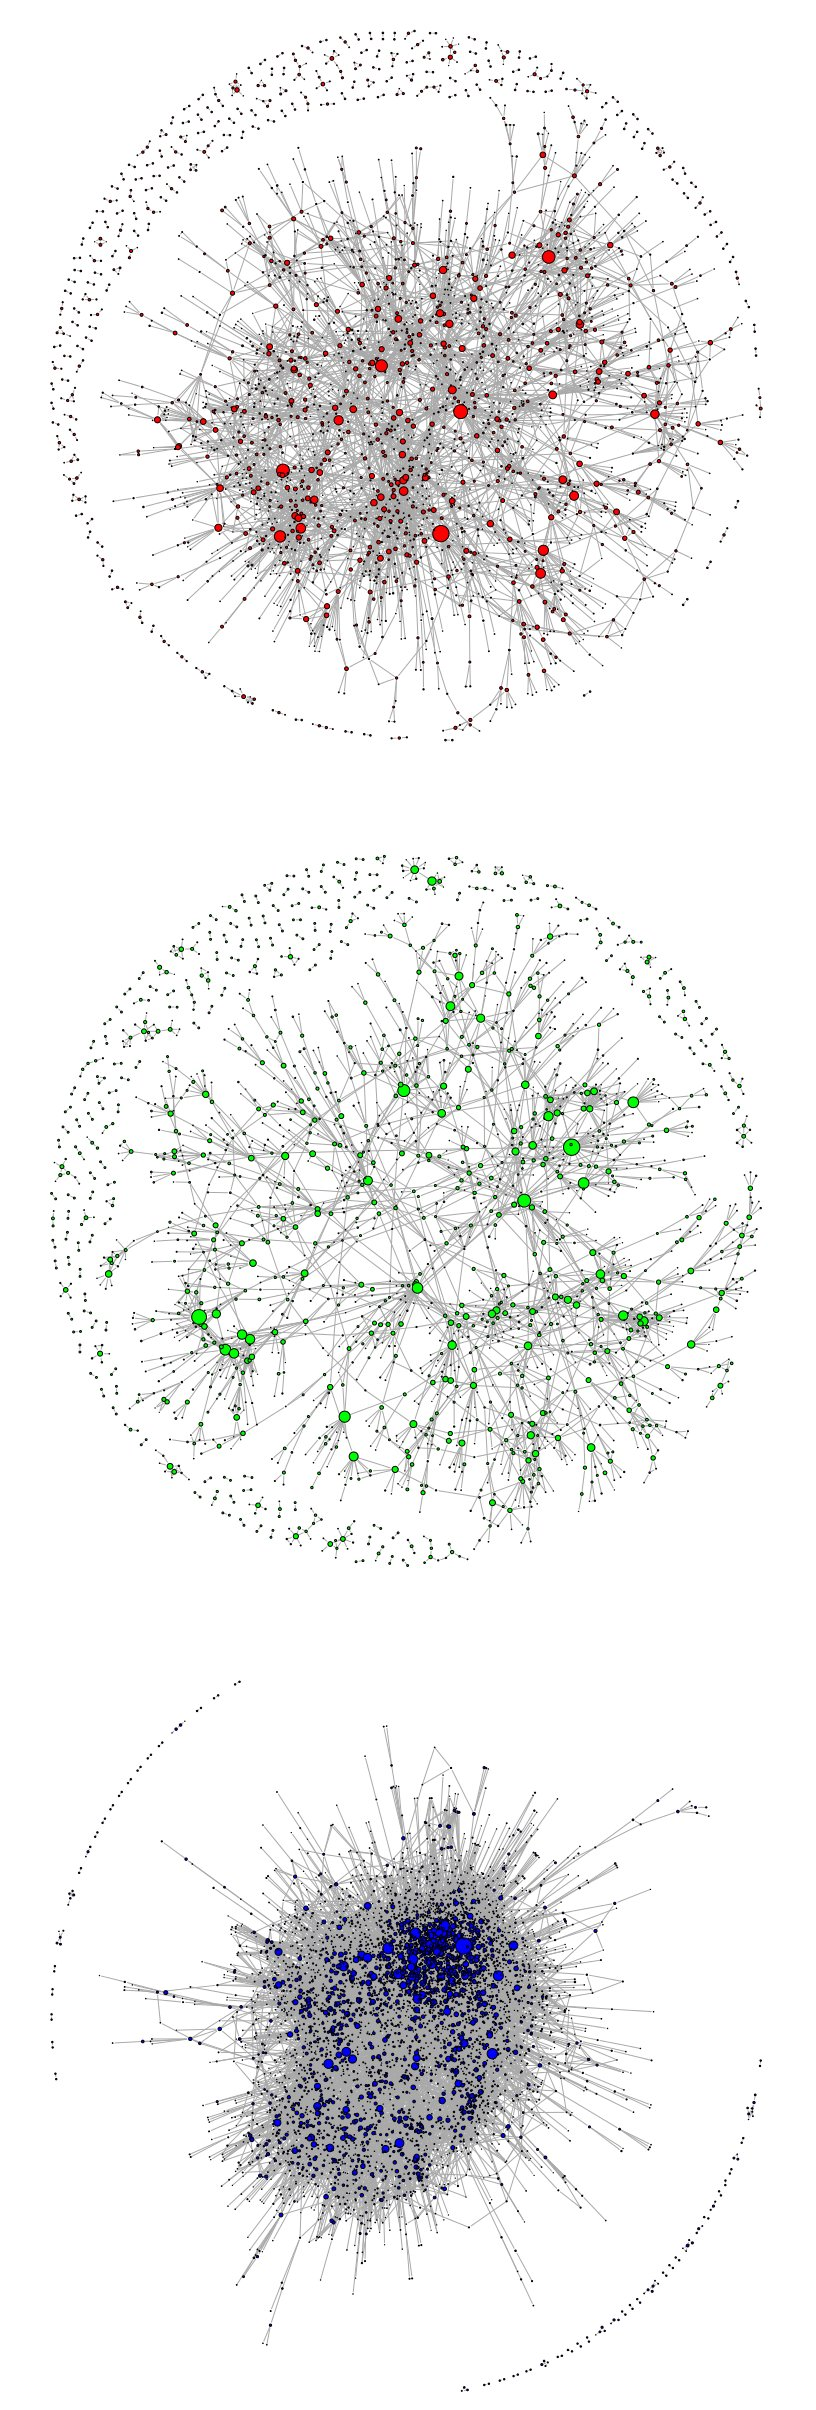
\includegraphics[height=7.90cm]{rede.jpg}
		\column{0.01\textwidth}
		\column{0.70\textwidth}
			\titlepage
	\end{columns}
	\addtocounter{framenumber}{-1}
\end{frame}
}

\end{document}

